\chapter*{3D Modelling and Animation}

\section*{3D Modelling}
The 3D model of the da Vinci robot was created in Autodesk 3DS Max. The robot needed to be modelled as realistic as possible and as such the program was chosen based on it's level of detail and built-in functions. However, due to the location and visitation possibilities of the da Vinci Si System it was not possible to capture every detail of the robot. As such, the robot is modelled partially from images taken, images on the internet, and memory. The robot was modelled with box modelling and was compared to a human model to ensure somewhat realistic sizes of the individual parts.

\begin{figure}[H]
	\centering
	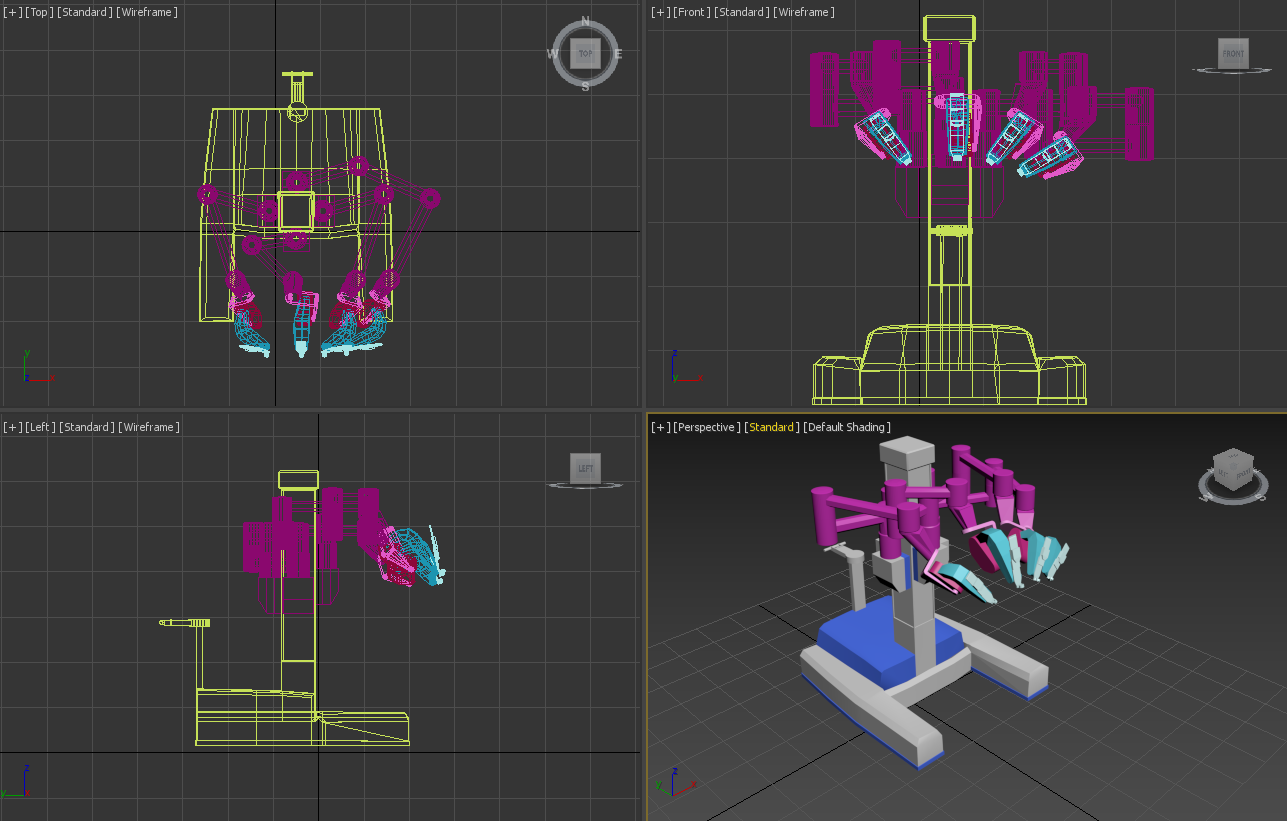
\includegraphics[width=0.75\textwidth]{ModelAnim/Max}
	\caption{The robot shown in Max' default workspace separated into four perspective views}
\end{figure}

After modelling finished the model was imported into Autodesk Maya which allows for easier rigging and animation. Maya is a tool that is tailored to animation whereas 3DS Max is primarily for modelling. Rigging the model was done according to where the robot is capable of rotating in real life.

\begin{figure}[H]
	\centering
	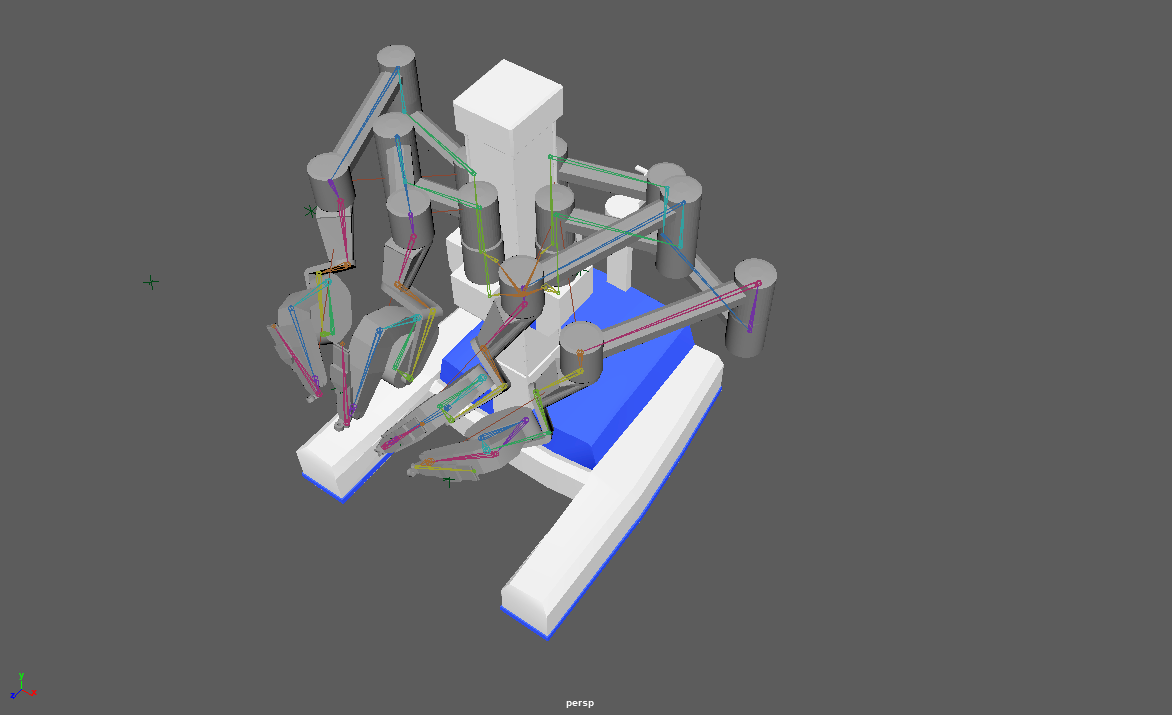
\includegraphics[width=0.75\textwidth]{ModelAnim/RobotMaya}
	\caption{The robot shown in Maya's default workspace indicating bones}
\end{figure}

\section*{3D Animation}
A 3D animation was created to ensure that realistic docking procedure could procede as a backup for the real-time interaction. In the case of using animation instead of interaction, a button would have to implemented in the scene to start the animation. As such, the robot would be in an initial "undocked" position and upon button press the robot would play the animation of docking. This animation could then be reverse to simulate undocking.

The animation was created in Autodesk Maya 2017, due to previous knowledge and its powerful animation tools. The robot had already been rigged in Maya for interaction in Unreal Engine 4, which allowed for quicker animation.

\begin{figure}[hpbt]
	\centering
	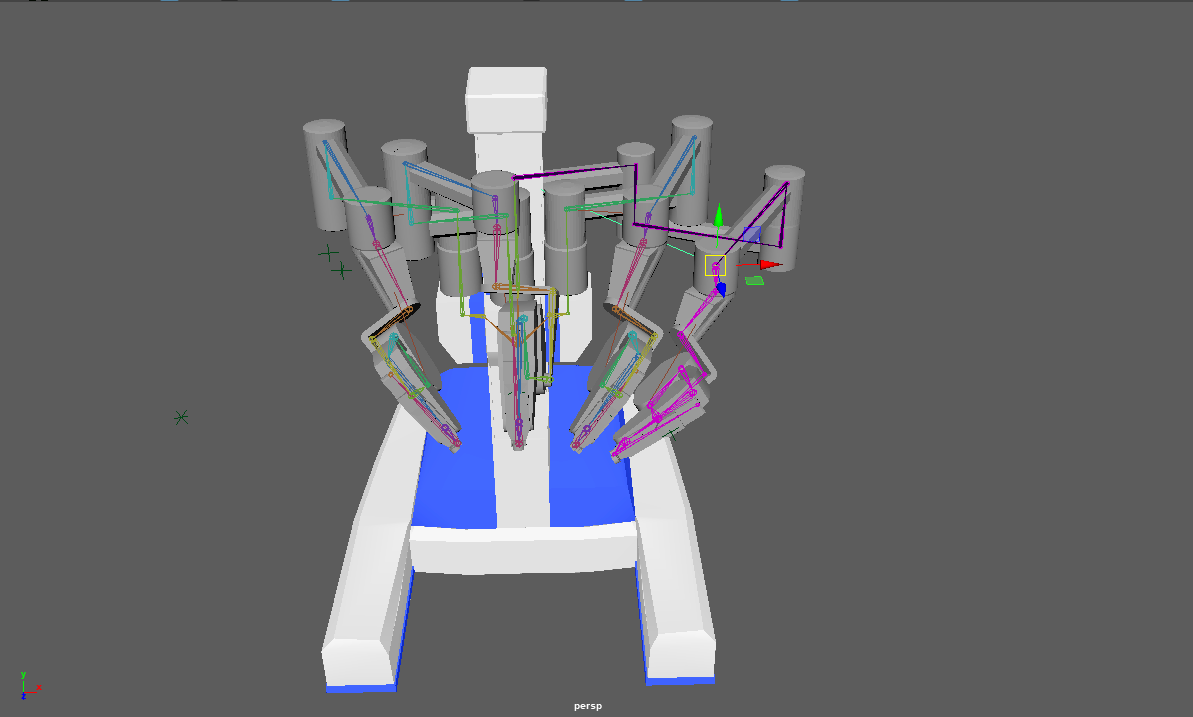
\includegraphics[width=0.3\textwidth]{ModelAnim/IK1}
	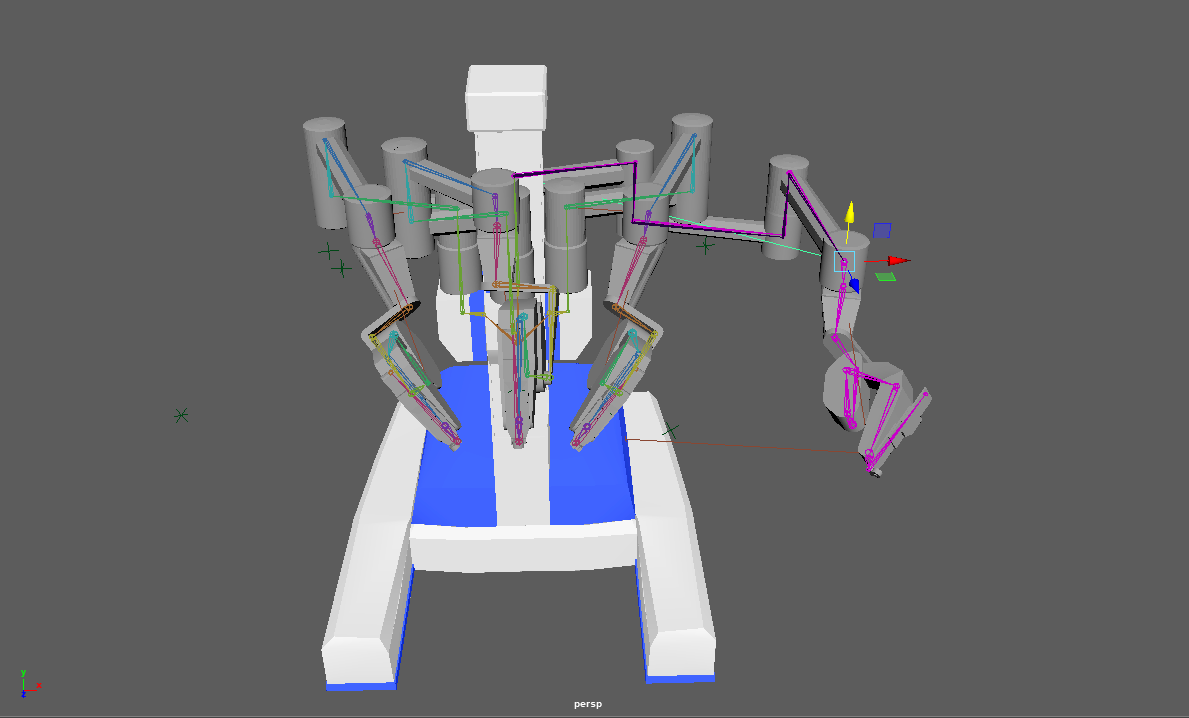
\includegraphics[width=0.3\textwidth]{ModelAnim/IK2}
	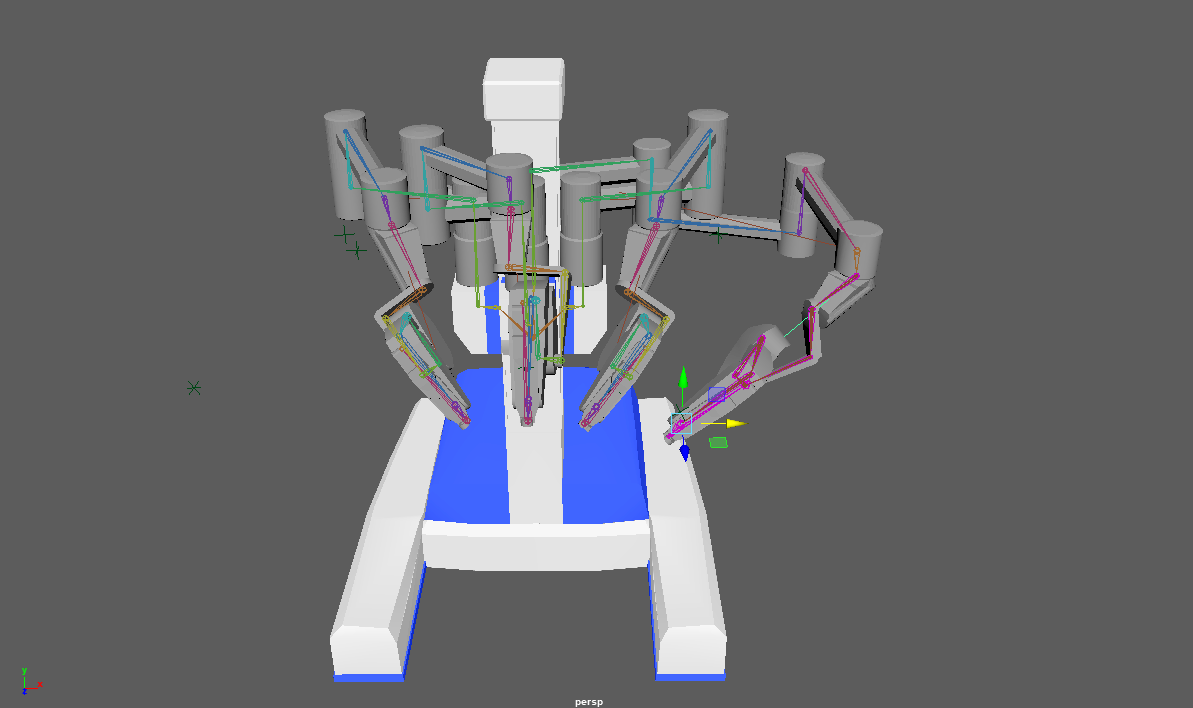
\includegraphics[width=0.3\textwidth]{ModelAnim/IK3}
	\caption{IK handles in Maya's workspace}
\end{figure}

Maya has two different IK solvers, named \textit{Single Chain IK solver} and \textit{Rotate Plane IK solver} (RP). This project uses the RP IK solver as it's end effector only tries to reach the position of the IK handle and not the orientation. This makes the bones' rotation more reliable. Furthermore, the entire bone chain can later be manipulated by the \textit{Twist Disc manipulator}.

\section*{The Scene}

The 3D modelled objects in the scene can be seen in \autoref{Fig:LUL}

\begin{figure}[hpbt]
	\centering
	\includegraphics[width=0.45\textwidth]{ModelAnim/RobotInGame}
	\includegraphics[width=0.45\textwidth]{ModelAnim/RobIRL}
	\caption{Left: Robot in the game. Right: Robot in real life}
	\label{Fig:LUL}
\end{figure}